\section{Diskussion}
\label{Diskussion}

Dieser Abschnitt diskutiert die zuvor beschriebenen Ergebnisse der Projektgruppe im Bezug zur initialen Zielsetzung \ref{Zielsetzung_und_Vorgehensweise}.

\paragraph{Die Generierung von Spielleveln}
Die Ziele bezüglich der Generierung von Spielleveln wurden erfolgreich umgesetzt.
Das Layout des Spiellevels wird prozedural mittels Space-Partitioning generiert und anschließend durch Terrain Transformationen in eine natürlich wirkende Welt verwandelt.
Die Welt besteht aus Räumen und Korridoren, die durch Gebirge voneinander getrennt werden.
Anders als bei einer typischen Generierung von Dungeons mittels Space-Partitioning, wird hierbei auf die Decke des Dungeons verzichtet, sodass die Welt aus offenen Arenen besteht, die durch Korridore miteinander verbunden sind.
In der Welt werden Spawn-Punkte für den Spieler, Kreaturen und Hindernisse platziert.
Die Hindernisse bestehen aus Pflanzen, die zur Laufzeit aus L-Systemen erzeugt werden.
Allgemein ist es möglich die Größe der Welt, die Anzahl an Räumen und die Anzahl an Spawn-Punkten für Hindernisse und Kreaturen einzustellen.
Der Schwierigkeitsgrad lässt sich durch kleinere Räume mit mehr Spawn-Punkten erhöhen.

\paragraph{Generierung der Monster}
Von Anfang an wurden bei der Generierung der Monster viele methodische Freiheiten gelassen. Damit konnten Beschränkungen bezüglich der Körperausprägungen vermieden werden. Während der Ausarbeitung sind dann die Zwei- und Vierbeiner in den Vordergrund gerückt, da diese auch für das Training bekannte und einfach erweiterbare Ansätze ermöglicht haben. Gleichzeitig ist schnell ersichtlich gewesen, dass die Auswahl der Körperteile eingeschränkt werden sollte, sodass die Komplexität der Kreaturen auf ein Minimum beschränkt wird und möglichst wenig Freiheitsgrade für das Training und Animieren der Kreaturen notwendig sind. Trotzdem ist es möglich, die entstandene parametrische Methode von Jona Heinrichs so zu erweitern, dass mit möglichst wenig Aufwand, Kreaturen mit einem noch größer variierenden Körperbau (z.B. Flügel, noch mehr Gliedmaßen, Acht-Füßler, etc.) entstehen können. Bei der parametrischen Methode ist es weiterhin wichtig, dass die Wertebereiche der Parameter passend zu der erwartenden Anatomie eines Zwei- und/oder Vierbeiners gewählt werden und dieser sich physikalisch korrekt animieren lässt.

Somit sind die Ziele, dass die Kreaturen-Erstellung Algorithmen-basiert ist und die innerhalb von Unity bereitgestellten Frameworks (z.B. Joints) verwendet werden sollten, erreicht worden. Für das Erreichen dieser Ziele, wurde sich ebenfalls so wie Anfangs angeschnitten, erfolgreich an dem Unity-ML-Agents-Walker orientiert.

Die folgenden Darstellungen in \ref{fig:finished_CG_2} \& \ref{fig:finished_CG_4} repräsentieren das fertige Ergebnis der Creature-Generator.

\begin{figure}[ht]
    \centering
    \begin{subfigure}[b]{0.2\textwidth}
        \centering        
        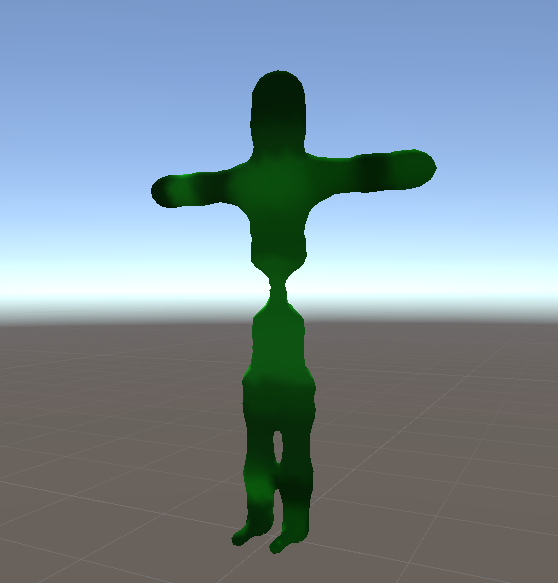
\includegraphics[width=\textwidth, height=\textwidth]{resources/img/Finished_Creatures_2/creature_1}
    \end{subfigure}
    \begin{subfigure}[b]{0.2\textwidth}
        \centering
        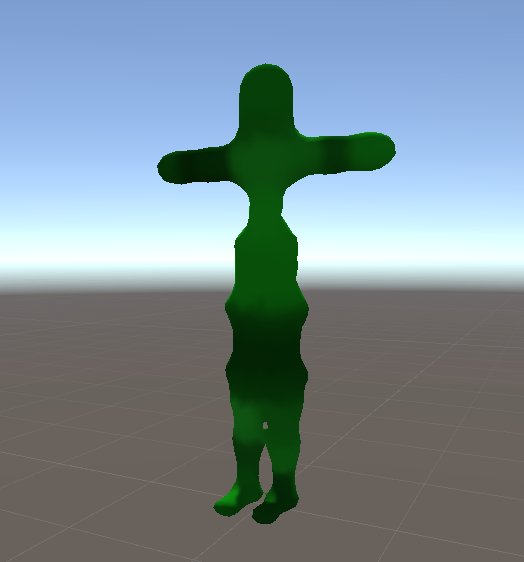
\includegraphics[width=\textwidth, height=\textwidth]{resources/img/Finished_Creatures_2/creature_2}
    \end{subfigure}
    \begin{subfigure}[b]{0.2\textwidth}
        \centering        
        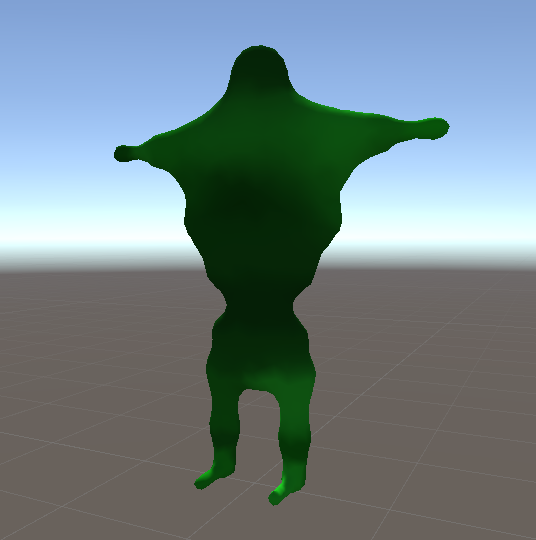
\includegraphics[width=\textwidth, height=\textwidth]{resources/img/Finished_Creatures_2/creature_3}
    \end{subfigure}
    \begin{subfigure}[b]{0.2\textwidth}
        \centering
        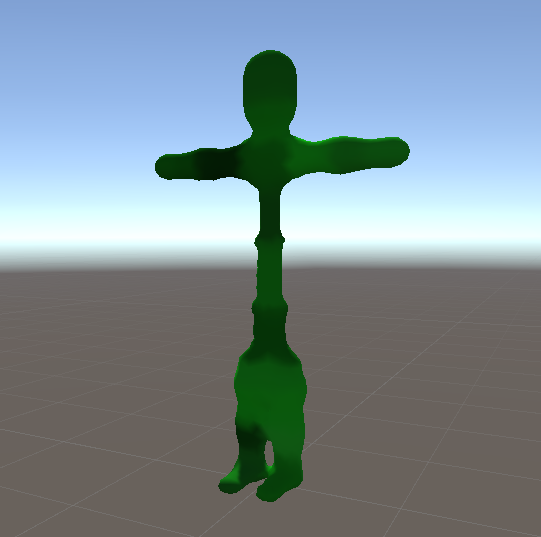
\includegraphics[width=\textwidth, height=\textwidth]{resources/img/Finished_Creatures_2/creature_4}
    \end{subfigure}
    \begin{subfigure}[b]{0.2\textwidth}
        \centering        
        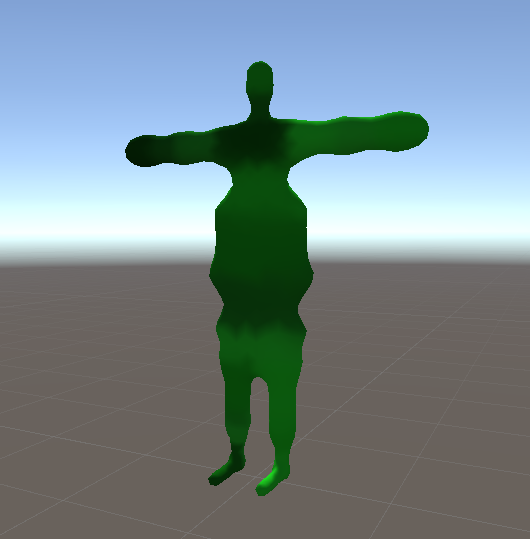
\includegraphics[width=\textwidth, height=\textwidth]{resources/img/Finished_Creatures_2/creature_5}
    \end{subfigure}
    \begin{subfigure}[b]{0.2\textwidth}
        \centering
        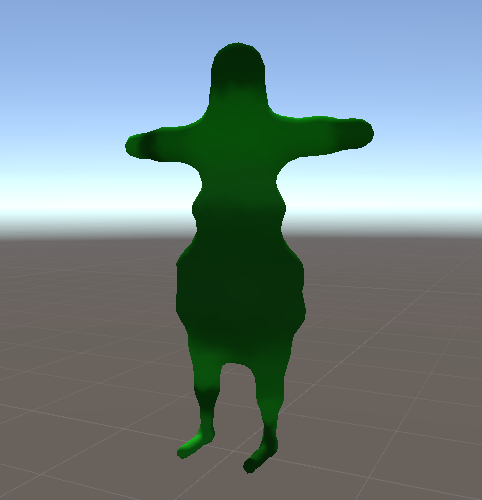
\includegraphics[width=\textwidth, height=\textwidth]{resources/img/Finished_Creatures_2/creature_6}
    \end{subfigure}
    \begin{subfigure}[b]{0.2\textwidth}
        \centering
        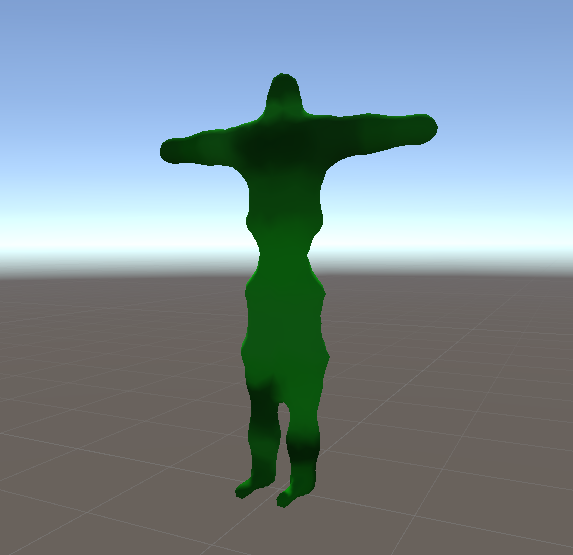
\includegraphics[width=\textwidth, height=\textwidth]{resources/img/Finished_Creatures_2/creature_7}
    \end{subfigure}
    \begin{subfigure}[b]{0.2\textwidth}
        \centering
        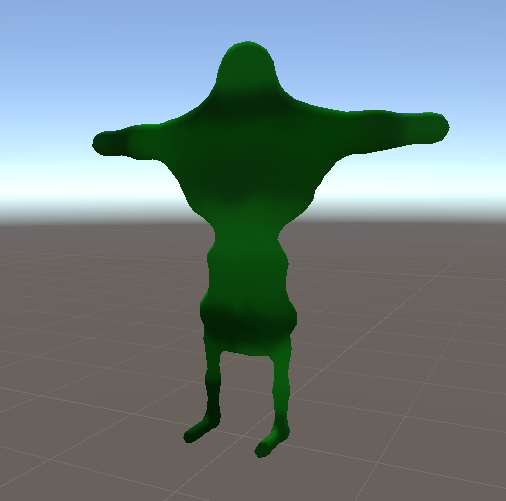
\includegraphics[width=\textwidth, height=\textwidth]{resources/img/Finished_Creatures_2/creature_8}
    \end{subfigure}
    \begin{subfigure}[b]{0.2\textwidth}
        \centering
        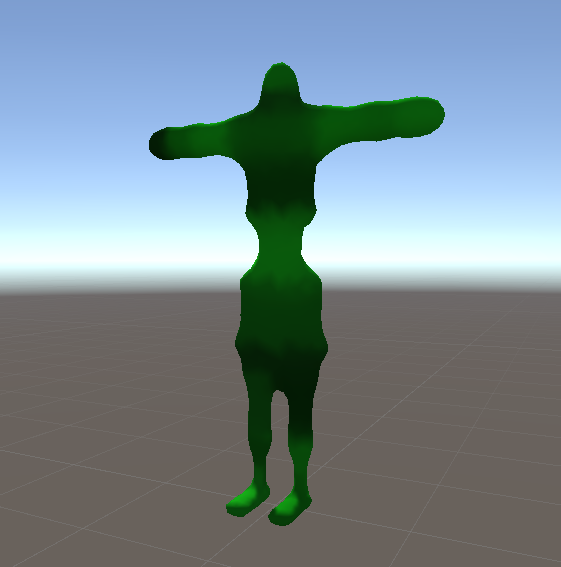
\includegraphics[width=\textwidth, height=\textwidth]{resources/img/Finished_Creatures_2/creature_9}
    \end{subfigure}
    \begin{subfigure}[b]{0.2\textwidth}
        \centering
        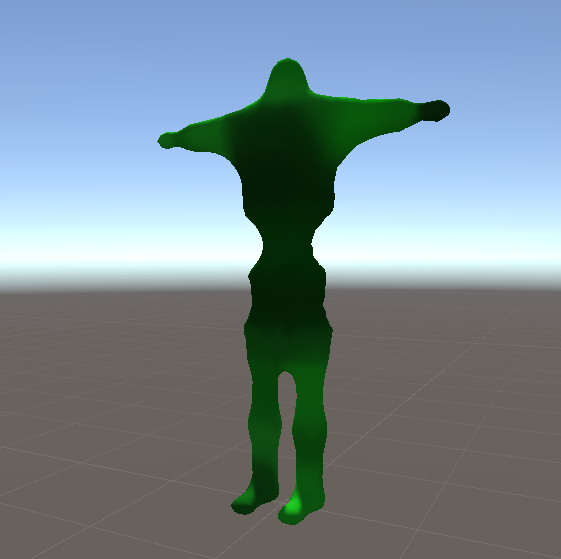
\includegraphics[width=\textwidth, height=\textwidth]{resources/img/Finished_Creatures_2/creature_10}
    \end{subfigure}
    \begin{subfigure}[b]{0.2\textwidth}
        \centering
        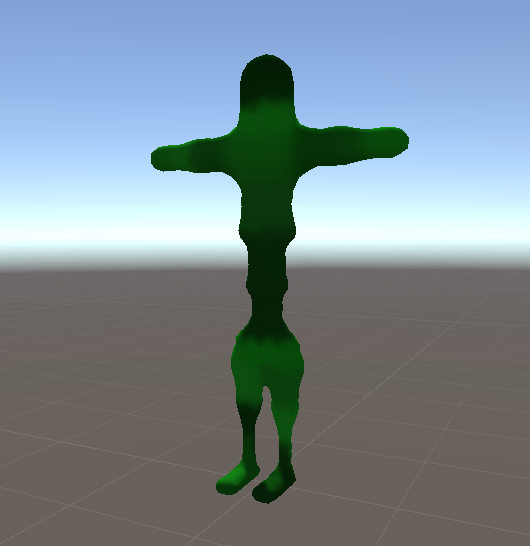
\includegraphics[width=\textwidth, height=\textwidth]{resources/img/Finished_Creatures_2/creature_11}
    \end{subfigure}
    \begin{subfigure}[b]{0.2\textwidth}
        \centering
        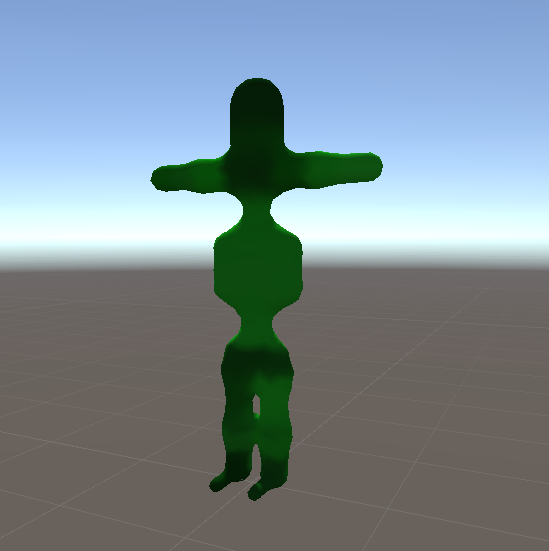
\includegraphics[width=\textwidth, height=\textwidth]{resources/img/Finished_Creatures_2/creature_12}
    \end{subfigure}
    \caption{Der fertige Creature-Generator Stand: Beispiele für Zweibeiner}
    \label{fig:finished_CG_2}
\end{figure}

\begin{figure}[ht]
    \centering
    \begin{subfigure}[b]{0.2\textwidth}
        \centering        
        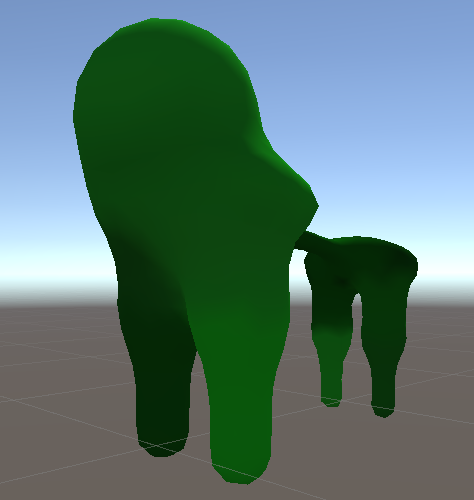
\includegraphics[width=\textwidth, height=\textwidth]{resources/img/Finished_Creatures_4/creature_1}
    \end{subfigure}
    \begin{subfigure}[b]{0.2\textwidth}
        \centering
        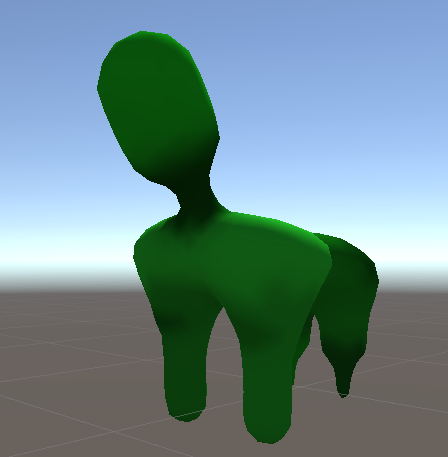
\includegraphics[width=\textwidth, height=\textwidth]{resources/img/Finished_Creatures_4/creature_2}
    \end{subfigure}
    \begin{subfigure}[b]{0.2\textwidth}
        \centering        
        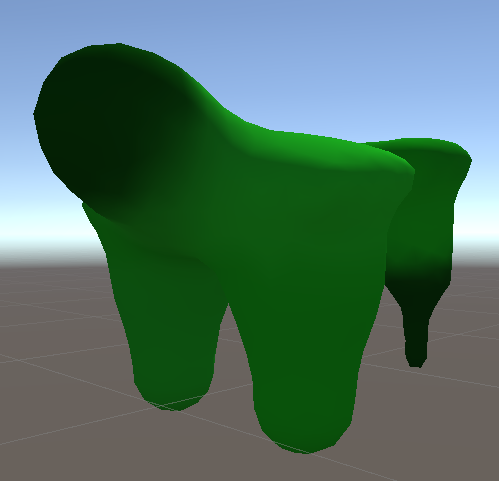
\includegraphics[width=\textwidth, height=\textwidth]{resources/img/Finished_Creatures_4/creature_3}
    \end{subfigure}
    \begin{subfigure}[b]{0.2\textwidth}
        \centering
        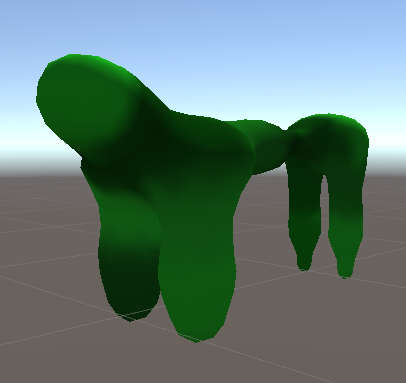
\includegraphics[width=\textwidth, height=\textwidth]{resources/img/Finished_Creatures_4/creature_4}
    \end{subfigure}
    \begin{subfigure}[b]{0.2\textwidth}
        \centering        
        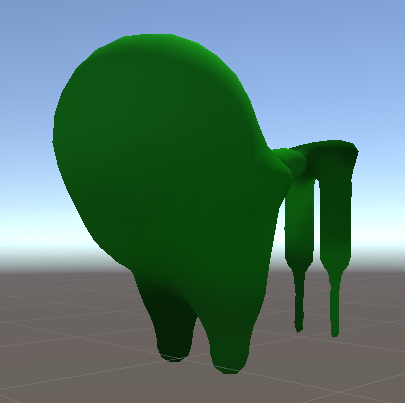
\includegraphics[width=\textwidth, height=\textwidth]{resources/img/Finished_Creatures_4/creature_5}
    \end{subfigure}
    \begin{subfigure}[b]{0.2\textwidth}
        \centering
        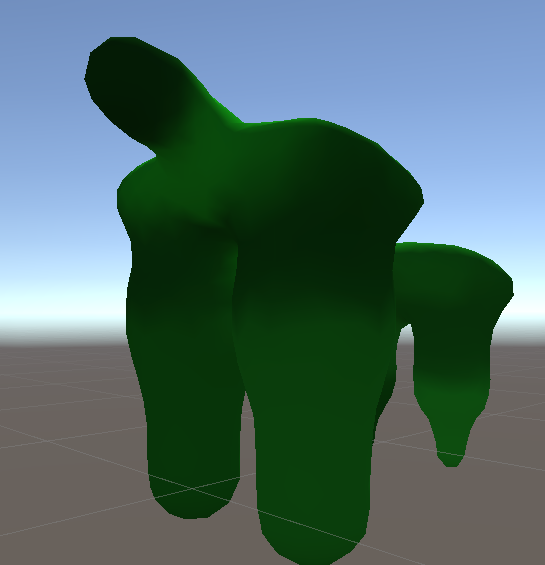
\includegraphics[width=\textwidth, height=\textwidth]{resources/img/Finished_Creatures_4/creature_6}
    \end{subfigure}
    \begin{subfigure}[b]{0.2\textwidth}
        \centering
        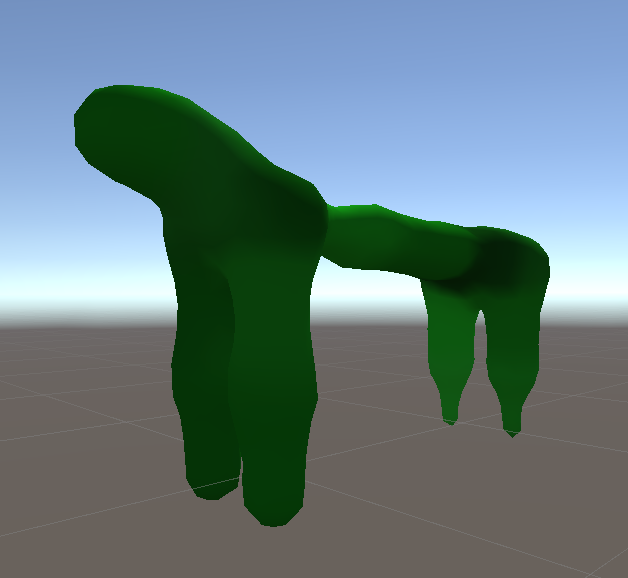
\includegraphics[width=\textwidth, height=\textwidth]{resources/img/Finished_Creatures_4/creature_7}
    \end{subfigure}
    \begin{subfigure}[b]{0.2\textwidth}
        \centering
        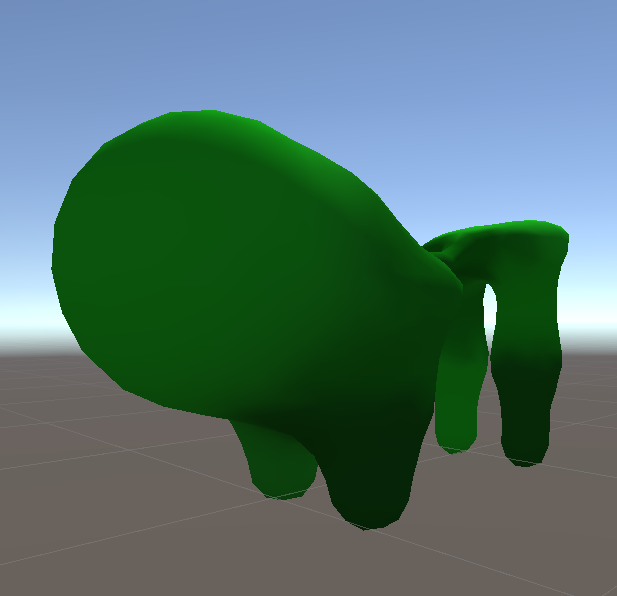
\includegraphics[width=\textwidth, height=\textwidth]{resources/img/Finished_Creatures_4/creature_8}
    \end{subfigure}
    \begin{subfigure}[b]{0.2\textwidth}
        \centering
        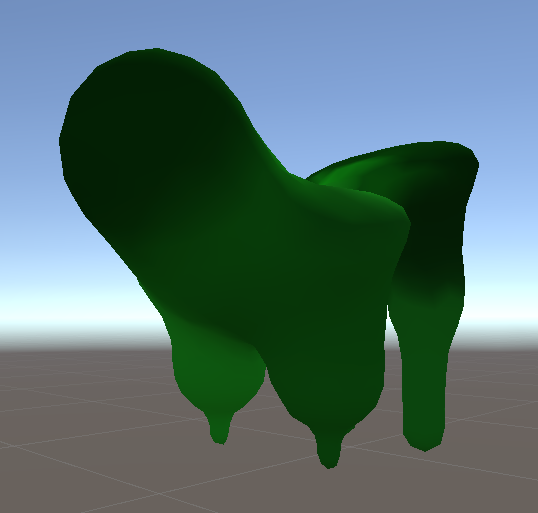
\includegraphics[width=\textwidth, height=\textwidth]{resources/img/Finished_Creatures_4/creature_9}
    \end{subfigure}
    \begin{subfigure}[b]{0.2\textwidth}
        \centering
        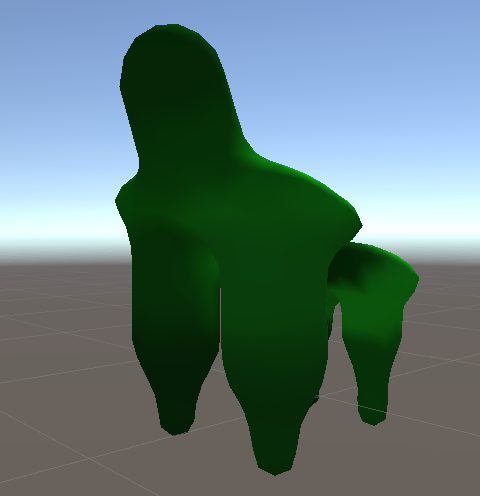
\includegraphics[width=\textwidth, height=\textwidth]{resources/img/Finished_Creatures_4/creature_10}
    \end{subfigure}
    \begin{subfigure}[b]{0.2\textwidth}
        \centering
        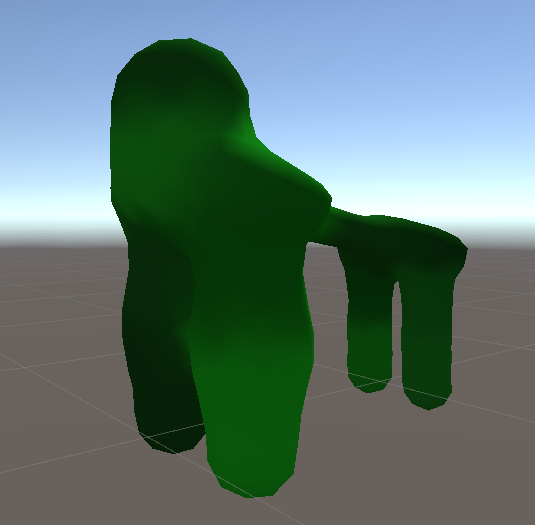
\includegraphics[width=\textwidth, height=\textwidth]{resources/img/Finished_Creatures_4/creature_11}
    \end{subfigure}
    \begin{subfigure}[b]{0.2\textwidth}
        \centering
        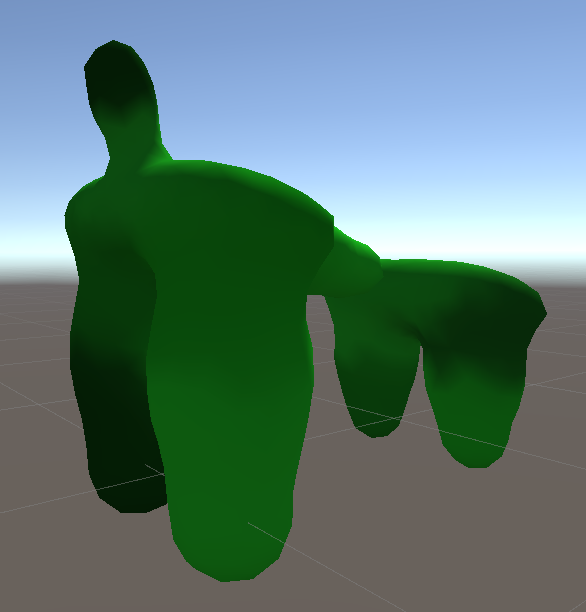
\includegraphics[width=\textwidth, height=\textwidth]{resources/img/Finished_Creatures_4/creature_12}
    \end{subfigure}
    \caption{Der fertige Creature-Generator Stand: Beispiele für Vierbeiner}
    \label{fig:finished_CG_4}
\end{figure}


\paragraph{Fortbewegung der Monster} \fup

Das festgelegte Minimalziel für die Fortbewegung der Monster war, dass die Animationen nicht manuell erstellt werden sollen. 
Stattdessen sollte mit Deep Reinforcement Learning ein Agent trainiert werden, der lernt die Monster zu bewegen, indem er Kräfte auf deren Joints ausübt.
Bei dem Versuch die ursprünglichen Vorstellung der Fortbewegung der Kreaturen umzusetzen traten allerdings einige Probleme auf.\\

Zum einen war das Trainieren der Fortbewegung von vollständig zufällig erstellten Kreaturen nicht möglich. 
In den ersten Trainingsdurchläufen wurde schnell klar, dass einige Kreaturen durch die Struktur ihres Körpers nicht dazu in der Lage waren sich stabil zu bewegen oder aufzustehen.
Ein Grund dafür kann zum Beispiel sein, dass die Bewegung einiger Joints zu weit eingeschränkt sind und die Agenten deswegen die mit diesen Joints verbundenen Körperteile nicht auf eine Art bewegen können, welche eine stabile Fortbewegung ermöglicht. Das selbe Problem trat auf, wenn eine Kreatur am Boden lag und im Zweifel ihre Arme und Beine nicht genug Freiheit hatten, um aus dieser Position herauszukommen.
Das entgegengesetzte Problem konnte auch auftreten, wenn die Freiheitsgrade zu hoch waren, da die Bewegungen dann nichts mehr mit der Fortbewegung von realen Tieren gemein hatten. Es war also notwendig die Parameter zur Generierung der Kreaturen einzuschränken, damit Fortbewegung möglich war.\\

Ein anderes Problem war die Stabilität der Fortbewegung. Die vierbeinige Kreatur, deren Trainingsergebnisse in dem Abschnitt \ref{ErgebnisseTraining} vorgestellt werden, ist nach dem Training in der Lage stabil zu laufen und auch wieder aufzustehen und kann deswegen in dem Spiel verwendet werden. 
Dies war allerdings nicht für alle generierten Vierbeiner der Fall, selbst wenn die zuvor erwähnten Einschränkungen an den Generator übergeben werden. Nach dem Training konnten zwar fast alle Vierbeiner laufen, aber in der Stabilität gab es große Variationen und einige der Kreaturen konnten nicht lernen aufzustehen. Aus diesem Grund wurde nur das eine vorgestellte Vierbeiner Modell dem Spiel hinzugefügt.\\
Die zweibeinige Kreatur ist nach dem absolvierten Training zwar in der Lage zu Laufen, aber dies ist insbesondere in Kurven sehr instabil. Dieses kann allerdings auch der gewählten Rewardfunktion geschuldet sein, da diese für das gesamte Training eine Geschwindigkeit vorgibt, welche der Agent einhalten sollte. Insbesondere in engen Kurven ist es für einen Zweibeiner aber aus Stabilitätsgründen effizient seine Geschwindigkeit zu verringern, wofür die Funktion den Agenten bestrafen würde. Das Problem mit der Stabilität ließe sich also eventuell entweder durch eine andere Rewardfunktion, die in Kurven langsamere Geschwindigkeiten erlaubt, oder eine andere Nav-Mesh Implementierung, die keine engen Kurven macht, lösen. Im Rahmen der Projektgruppe war allerdings keine Zeit mehr diese Vermutungen zu überprüfen.\\
Die Zweibeiner hatten außerdem Probleme mit dem aufstehen. Nach dem Training konnte die Kreatur zwar aus dem liegen wieder in den Stand kommen, aber sie blieb danach nicht stehen, sondern fiel wieder zu Boden. Diese Kombination aus instabilem Laufen mit häufigen umfallen in Kurven und der Unfähigkeit aufzustehen macht die Zweibeiner ungeeignet für eine Verwendung in dem Spiel. Daher wurde entschieden keine zweibeinigen Monster in das Spiel zu integrieren. \\

Abschließend lässt sich also sagen, dass das zu Beginn festgelegte Minimalziel erreicht wurde und für die exemplarischen Kreaturen Modelle trainiert wurden, dass diese zum laufen und aufstehen verwenden können. Außerdem wurde ein einfacher Mechanismus implementiert, der Anhand einer übergebenen Bedingung entscheidet, ob die Kreatur im nächsten Schritt das Modell zum laufen und das zum aufstehen verwenden soll. \\
Die Umsetzung der weiterführenden Ideen ist allerdings zum größten Teil gescheitert. 
Insbesondere die Ansätze zur Diversifikation der Generierung, ein Agent der allen Kreaturen beibringen kann zu laufen, und zur Generalisierung des Trainings, ein Modell welches von allen Kreaturen mit ähnlichen Skeletten zum laufen verwendet wird, konnten nicht umgesetzt werden.

\paragraph{Handlungsempfehlungen}
Die Ergebnisse der Projektgruppe zeigen, dass das Generieren von Bewegungsanimationen für prozedural generierte Skelette durch Reinforcement Learning möglich ist. Für die Zwei- und Vierbeiner Kreaturen werden vielversprechende Eregbnisse erzielt, wobei insbesondere die Ergebnisse der Vierbeiner ohne größere Einschränkungen im entwickelten Spiel einsetzbar sind.
Allerdings unterliegen die Ergebnisse diversen Einschränkungen, die in den vorherigen Abschnitten detailliert beschrieben wurden. Diese Einschränkungen stehen teilweise im Widerspruch zu den initialen Erwartungen, dass Reinforcement Learning basierte Methoden genereller und mit geringerem Aufwand einsetzbar sind, als traditionelle Keyframe Methoden zur Charakteranimation. Der Aufbau einer Umgebung, die die Anwendung von Reinforcement Learning erlaubt, ist mit großem Aufwand verbunden. Die Umgebung muss die Zielumgebung (d.h. das tatsächliche Spielumfeld der Kreaturen) so modellieren, dass die gelernten Bewegungsanimationen auch im fertigen Spiel einsetzbar sind. Um realistische Animationen zu trainieren, die an die Bewegung echter Lebewesen erinnern, müssen entsprechende Einschränkungen in die Rewardfunktion integriert werden. Die Modellierung dieser Einschränkungen erfordert tiefgehendes Wissen über die zu trainierenden Kreaturen, um beispielsweise auf Positionen der Knochen zuzugreifen. Außerdem ist die Entwicklung einer funktionierenden Rewardfunktion nicht trivial, da die tatsächlichen Effekte der einzelnen Rewards nicht eindeutig sind. Somit vereinfacht die hier beschriebene Anwendung von Reinforcement Learning zur Charakteranimation diese nur bedingt.
Sind die Einschränkungen und initialen Hindernisse überwunden und es existieren eine Modellumgebung, die für das Training verwendet werden kann, sowie Rewardfunktionen für die gewünschten Bewegungen, können durch Reinforcement Learning relativ schnell Animationen für zusätzliche Charaktere generiert werden. Je nach Komplexität der Umgebung und der Skelette, und abhängig von der verfügbaren Hardware, dauert ein Trainingsprozess trotzdem mehrere Tage, sodass potenziell auch Keyframe Animationen mit ähnlichem Zeitaufwand erstellt werden könnten. Die Generierung von Animationen für neue Kreaturen in Echtzeit ist nicht möglich. Es ist außerdem nicht garantiert, dass neu generierte Kreaturen mit den definierten Rewardfunktionen einen vergleichbaren Lernerfolg haben. Selbst mit den starken Einschränkungen bei der Generierung neuer Kreaturen im Rahmen der Projektgruppe, erzielt nicht jede Kreatur einen vergleichbaren Lernerfolg. Um das Problem der Laufzeit der Trainingsdurchläufe zu umgehen und verschiedenartige Kreaturen zu unterstützen, bietet sich ein generalisiertes Training an, dass Bewegungsanimationen für verschiedenartige Kreaturen lernt. Damit könnten sogar in Echtzeit neue Kreaturen generiert und animiert werden. Die Versuche zur Generalisierung während dieser Projektgruppe führten aufgrund der hohen Komplexität jedoch nicht zu erfolgreichen Ergebnissen.

Die Charakteranimation durch Reinforcement Learning mit den in diesem Bericht beschriebenen Methoden erzielt interessante und teilweise vielversprechende Methoden. Für Einsatzgebiete, die flexible und unrealistische Animationen (z.B. für die Animation von Monstern), den initialen Entwicklungsaufwand und die laufenden Hardwarekosten erlauben, lassen sich durch Reinforcement Learning vielfältige Animationen generieren.

